\chapter{Monte Carlo Simulation}
\label{MCS}
\graphicspath{{chapter-7/Images/}}

\section{Introduction}
Monte Carlo is a simulation technique wherein uncertain inputs to a simulation model are represented in the form of a probability distribution. When we talk about observing the trajectories of multiple particles around a binary system, we want to observe all possible scenarios in which these particles could be lofted from the surface of the asteroid and then analyze the corresponding long or short-term behavior of the particles in orbit. In this regard, Monte Carlo simulations will turn out to be a useful tool. It will be utilized in generating multiple debris particles at the surface of the asteroid by basically generating random initial state vectors (position and velocity) from a reasonable probability distribution for the third body in the three-body problem. These particles will then be propagated in the three-body simulator to record its orbit.

It is assumed that the surface debris is lofted off the surface of the asteroid due to an impact by a spacecraft or its constituent as part of an exploration program. This will result in a crater on the asteroids surface from where the debris shall be lofted. Since we are modeling the asteroids as polyhedrons, we can consider certain multiple adjacent facets on the polyhedron from where we will assume that the debris is lofted from. Thus these facets will enable us to put a boundary on the probability distribution from which we can sample random values for the position components of the initial state vector, thereby ensuring that the initial vector is from within a designated surface area on the asteroid and not elsewhere. For the velocity components, we will follow a similar process but for the first set of simulation the probability distribution shall be bounded between a velocity of 0 and the escape velocity. The second set of simulation could involve increasing the upper bound from the escape velocity by a certain constant factor to observe if the perturbations could play a more significant role in the dynamical environment around the asteroid than the latter's gravitational force itself (this phenomenon will also be analyzed for in the first set of simulations as well), such as bringing back the particle back to the asteroid's surface despite having a higher than escape velocity. Thus in this manner we will be able to simulate the various, if not all, conditions in which a particle can be lofted from the surface. The Monte Carlo simulation will help us in determining the range of all possible outputs along with the likelihood of each occurring.

Now that we have presented a rationale for using Monte Carlo methods, this chapter will further discuss the way in which we can produce a random value generating function from a given probability density function of our choice following which we will discuss how we can sample random values using the generating function.

\section{Random Value Generating Function}
We need a random value generating function for each component of the initial state vector to run the Monte Carlo simulation. To do that we first need a probability density function $f(x)$, then from this we will obtain the distribution function $F(x)$. The random value generating function $G(F(x))$ will then generate the random value as $x = G(f(x))$ \cite{monteweb}.

We will take a general example and explain the whole process of obtaining $G(F(x))$. Consider a sinusoidal probability density function, shown in \Cref{fig:pdf}, as follows \cite{monteweb}:
%
\begin{figure}[h]
\centering
\captionsetup{justification=centering}
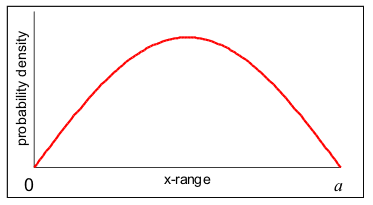
\includegraphics[scale=1]{pdf.png}
\caption{Sinusoidal probability density function \cite{monteweb}.}
\label{fig:pdf}
\end{figure}
\FloatBarrier
%
\begin{equation}
f(x) = b \sin \left( \frac{\pi x}{a} \right)
\end{equation}
%
where $a$ and $b$ are two constants and x is the random value. From this the cumulative distribution function is obtained as follows \cite{monteweb}:
\begin{equation}
F(x) = \int_0^x b \sin \left( \frac{\pi x}{a} \right) dx = \frac{ab}{\pi}(1 - \cos(\pi x/a))
\end{equation}
%
The area under the probability density function must be equal to unity. The user can set the value of the constant $a$ and then the value of $b$ can be obtained such that $F(a) = 1$ \cite{monteweb}:
\begin{equation}
F(a) = 1 = (ab/\pi) (1 - \cos(\pi)) = 2ab/\pi
\end{equation}
%
Thus from the above expression, the value of $b$ comes out to be $b = \pi/2a$. Then $F(x)$ becomes \cite{monteweb}:
\begin{equation}
F(x) = 0.5 (1 - \cos(\pi x/a))
\end{equation}
%
Now we can get the random value generating function from $G(F(x)) = x$ by rearranging the terms such that \cite{monteweb}:
\begin{equation}
x = (a/\pi) \cos^{-1} (1 - 2.F(x)) = G(F(x))
\end{equation}
%
Thus by choosing an appropriate probability density function for each component of the initial state vector of the third particle in the three-body problem, we can generate appropriate random values to initiate the simulation.

\section{Random Value Sampling}
Once we have the distribution function and the corresponding generating function, we need a way in which we can efficiently sample the random value. For this purpose, we shall use a sampling technique called the Latin Hypercube sampling. In this method the distribution function is divided into equal $n$ intervals where $n$ is the number of iterations we want to perform in the Monte Carlo simulations. A graphical representation of this is given in \Cref{fig:lhs} \cite{monteweb}:
%
\begin{figure}[h]
\centering
\captionsetup{justification=centering}
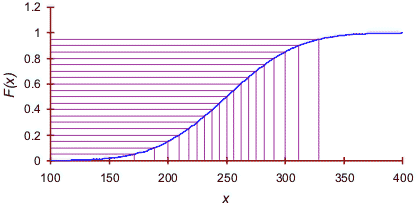
\includegraphics[scale=1]{lhs.png}
\caption{Equal intervals in Latin Hypercube sampling \cite{monteweb}.}
\label{fig:lhs}
\end{figure}
\FloatBarrier
%
The iterations begin by randomly selecting one of the intervals out of the $n$ intervals. A second random number is then used to determine where within the selected interval would the value of $F(x)$ would lie. Using this value of $F(x)$ the random value $x = G(F(x))$ is obtained. The integration process continues and whatever interval was used earlier is marked so that it is not used again. This avoids repetition of iterations \cite{monteweb}.

\section{Conclusion}
This chapter provided the mathematical basis for the use of Monte Carlo simulation in a generalized manner. In the introduction we also presented the motive for using this simulation technique and how this technique would be applied to generate multiple debris particles at the surface of the asteroid. Another simulation technique which was not discussed in this chapter, called the grid-search or enumerative technique, involves a systematic search through a predefined model space (in our case the model space would contain the initial values for position and velocity of the orbiting particle) and then the evaluation of the dynamical model for each of the grid-searched values \cite{grid_monte}. For the astrodynamics problem of a particle orbiting around an asteroid, a grid-search based method will not be practical because the model space or the search space will be very large. On the other hand, the Monte Carlo method is a random search method wherein the search space can be narrowed by defining a probability distribution function from which the model parameters (i.e. the initial conditions) are sampled from \cite{grid_monte}.

Monte Carlo simulation will be necessary in analyzing all "what-if" situations such as "what if the particle has an initial velocity less than the escape velocity" or "what if the particle is deployed from the pole or the equator of the asteroid" and so on. Once a dynamics simulator is set up, it is very important that we exploit the simulator to assess every possible outcome and to be able to do this, we need the Monte Carlo simulation technique.
